\documentclass[12pt]{article}
\usepackage{pagestyle}

\begin{document}
\thispagestyle{empty}

{\scshape ML } \hfill {\scshape \large Lecture 6 - Beyond Linear Models} \hfill {\scshape 20.02.2024}
 
\smallskip
\hrule
\bigskip

%table of contents 
\tableofcontents

\section{Neural Networks (NN) and Support Vector Machines (SVM)}

Neural networks and support vector machines (SVM) both build on the idea of making a linear model more powerful by expanding features.

\subsection{NN}

A simple neural network is a two-layer feedforward network. It functions as a feature extractor followed by a classifier. We don't choose the extended features but we learn them, together with the weights of the classifier. \smallskip

\textbf{For example} in handwriting recognition each image is represented by a vector of pixel values, not any chosen feature. The network they learnes to recognize consistent features among the images and then classifies them based on these features to some target, for example output nodes labelled 0-9.


\subsection{SVM}

SVMs don't learn expanded features, they have to be chosen, but they use a \textit{kernel function} to allow us to fit a linear model to very high-dimensional feature space without having to pay for compute all expanded features and storing them in memory.

\subsection{NN and SVM summary}

\begin{figure}[!h]
    \centering
    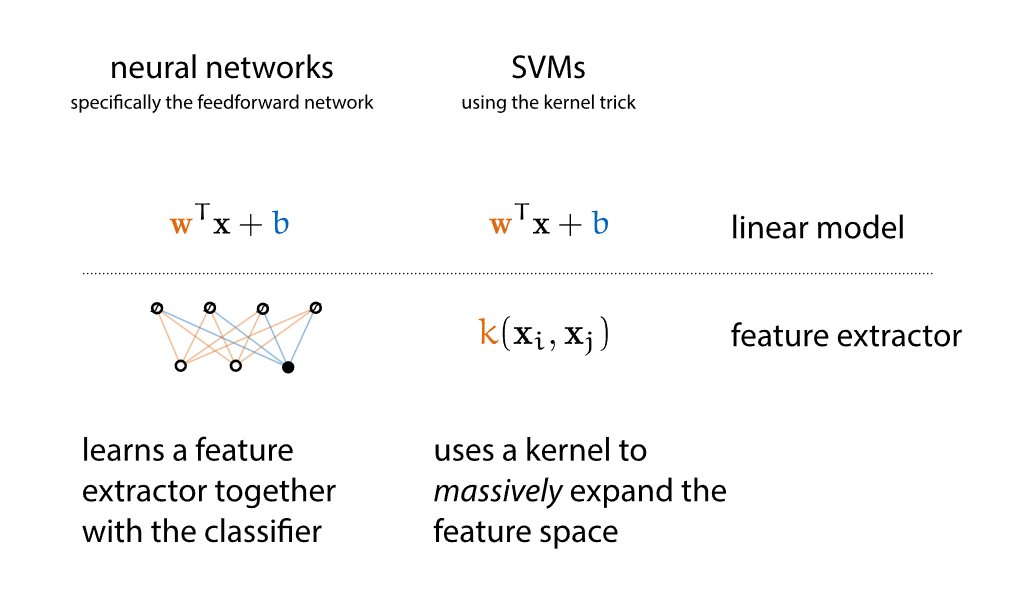
\includegraphics[width=0.6\textwidth]{assets/svmandnn.png}
\end{figure}

\subsection{Perceptron}

\begin{definition}[Perceptron]
    A percetron is a machine learning model with a number of inputs, generally $x_1, x_2, \ldots, x_n$, and a single output. The output is a step function of a linear combination of the inputs. Visually we can represent this as follows: 
    \begin{figure}[!h]
        \centering
        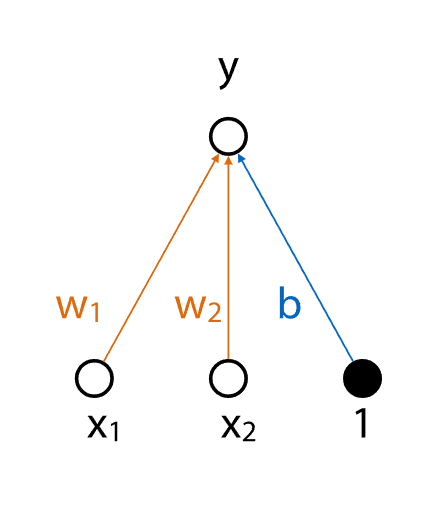
\includegraphics[width=0.2\textwidth]{assets/basicperceptron.png}
    \end{figure}
    Mathematically, the output $y$ is given by:
    \[ y = \begin{cases} 1 & \text{if } \mathbf w \cdot  \mathbf x + b > 0 \\ 0 & \text{otherwise} \end{cases} \]
    where $\mathbf w$ is the weight vector, $\mathbf x$ is the input vector, and $b$ is the bias.
\end{definition}

\subsubsection*{Simple composition}

A simple composition of neurons does \textit{not} make them more powerful. The function $y$ generated by a composition of neurons is still a linear function of the inputs. To combine percetrons in a way more expressive than a single perceptron there needs to be non-linearity introduced in the form of \textbf{actiation functions}.

\subsection{Activation functions}

\begin{definition}[activation function]
    Activation functions are used to introduce non-linearity into the output of a neuron. The most common activation functions are the sigmoid, and nowadays the rectified linear unit (ReLU).
\end{definition}

\begin{multicols}{2}
    \subsubsection*{Logistic sigmoid}
    For logistic sgimoid the inputs can be any value and the output is constrained to [0, 1].
    \[ \sigma(x) = \frac{1}{1 + e^{-x}} \]
    \columnbreak
    \subsubsection*{ReLU}
    The ReLU function is defined as the max of 0 and the input. If the input is 0 or negative, the output is 0, otherwise the output is the input.
    \[ \text{ReLU}(x) = \max(0, x) \]
    \vfill\null
\end{multicols}

In terms of the perceptron all we are doing is feeding the summed outputs of the perceptrons through an activation function. 

\begin{figure}[!h]
    \centering
    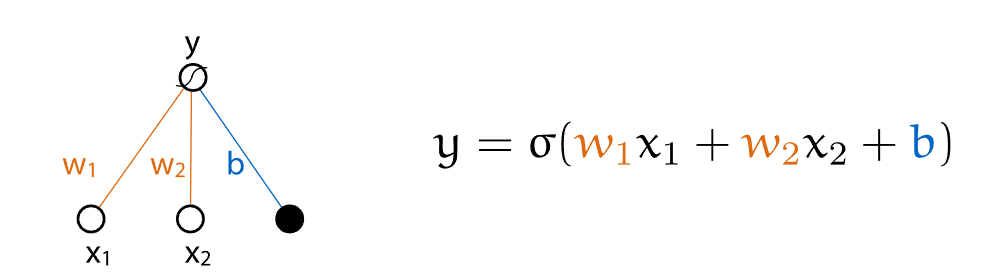
\includegraphics[width=0.5\textwidth]{assets/perceptronwithact.png}
\end{figure}

\subsection{Feedforward Neural Networks}

\begin{definition}[Feedforward Neural Network]
    A feedforward neural network is a network of neurons where the output of each neuron is fed as input to the next layer of neurons. The first layer is the \textbf{input layer}, the last layer is the \textbf{output layer}, and any layers in between are called \textbf{hidden layers}.
\end{definition}

FNN's are also known as multilayer perceptrons since they are a multilayer composition of perceptrons which use activation functions to introduce non-linearity in the hidden layers. 
\smallskip
Some properties of FNN's:
\begin{itemize}[leftmargin=*, noitemsep]
    \item There are no cycles
    \item Nodes in the same layer are not connected
    \item Each layer is fully connected to the previous layer
\end{itemize}

\subsubsection*{Pseudocode example}
\begin{multicols}{2}
    
    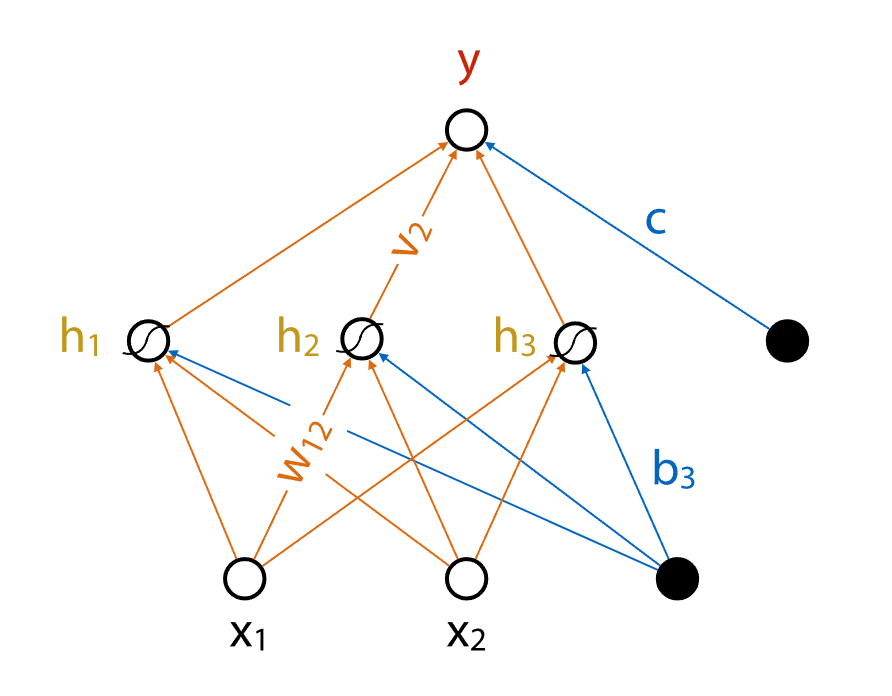
\includegraphics[width=0.4\textwidth]{assets/FNN.png}

    \columnbreak

    \begin{lstlisting}
    for j in 1 ... 3: 
        for i in 1 ... 2:
            $k_j$ += $w_{ij} \cdot x_i$
        $k_j$ += $b_j$

    for i in 1 ... 3:
        $h_i$ = $\sigma(k_i)$

    for i in 1 ... 3:
        y += $h_i \cdot v_i$
    y += $c$

    loss = $(y - \text{target})^2$
    \end{lstlisting}
\end{multicols}

Some notes regarding this model: 
\begin{itemize}[leftmargin=*, noitemsep]
    \item $k_j$ here represents the inputs to the hidden layer nodes (the activation functions), formally we can write $k_j = \sum_{i=1}^3 w_{ij} \cdot x_i + b_j$. As an example: 
    \[
        k_2 = w_{21} \cdot x_1 + w_{22} \cdot x_2 + b_3
    \]
    \item $b_j$ is the constant bias term for the hidden layer nodes
    \item In the above example we are using the sigmoid activation function, $\sigma(k_i)$, expressed fully: 
    \[
        h_i = \sigma(k_i) = \sigma\left(\sum_{i=1}^3 w_{ij} \cdot x_i + b_j\right)
    \]
    \item The loss function is the squared difference between the output and the target, the partial derivative of which can be used to update the weights.
    \item If we where to add another hidden layer the pseudocode for the first hidden layer would be similar to that of the input layer, it would look roughly as follows 
    \begin{multicols}{2}
        \begin{lstlisting}
    # same as before

    # for each node in the hidden layer
    for j in 1 ... 3: 
        for i in 1 ... 2: 
            $h_j$ += $w_{ij} \cdot \sigma(k_i)$
        $h_j$ += $b_j$

    # last hidden layer
    for i in 1 ... 3:
        $h_i$ = $\sigma(k_i)$

    # same as before
        \end{lstlisting}
        \columnbreak
        Mathematically speaking we are doing the same thing as for the input layer but simply replacing the input term $x_i$ with the output of the previous hidden layer, $\sigma(k_i)$.
        \[
            h_j = \sigma\left(\sum_{i=1}^3 w_{ij} \cdot \sigma(k_i) + b_j\right)  
        \]
        Im assuming here that we include the bias term for each hidden layer.
    \end{multicols}
\end{itemize}

\subsection{Regression FNN model}
\begin{definition}[Regression FNN]
    A regression feedforward neural network is an FNN where we need one output node without an activation function. The first layer can be seen as learning the feature expansion and the second layer is a linear regression in the expanded feature space.
\end{definition}

\begin{multicols}{2}
    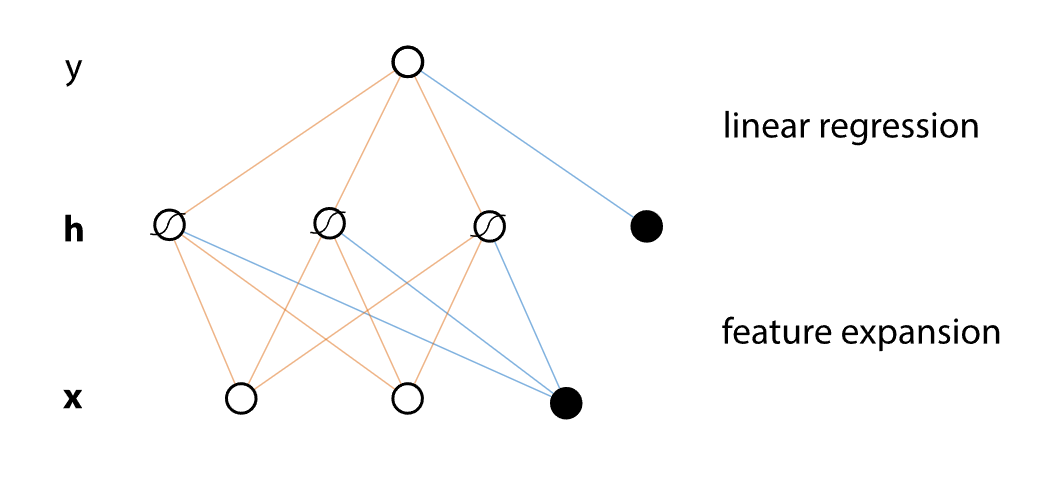
\includegraphics[width=0.5\textwidth]{assets/regFNN.png}
    \columnbreak \\ 
    The number of hidden nodes is a hyperparameter.
    \begin{itemize}[leftmargin=*, noitemsep]
        \item $\uparrow$ number of hidden nodes 
        \\ $\Rightarrow$ more expressive model 
        \\ $\Rightarrow$ more prone to overfitting; harder to train; more expensive to compute
    \end{itemize}
    The one thing you should always do is have a wider hidden layer than the input layer.
\end{multicols}

\subsection{Classification FNN model}

Classification FNN's are similar in structure to regression FNN's but with a different output layer.

\begin{definition}[Binary Classification FNN]
    A binary classification feedforward neural network is an FNN where nowadays we use the sigmoid activation function on the output and interpret this as the probability of the input being in a class given the input. Formally we say that: 
    \[
        P(y = 1 \mid \mathbf x) = \sigma\left(\sum_{i=1}^n w_i \cdot h_i + c\right)  
    \]
    
\end{definition}

\begin{definition}[Multiclass Classification FNN]
    A multiclass classification FNN has a single output node for each class (e.g. labelled 0-9 for handwriting recognition), where we ensure they are all positive and sum to 1. Allowing us to interpret them as class probabilities. This is done by using the softmax activation function on the output layer.
    \begin{multicols}{2}
        \begin{align*}
            o_i & = \mathbf w^\intercal \mathbf h + b \\ 
            P(y_i = i\mid \mathbf{x}) & = \frac{\exp (o_i)}{\sum_{j=1}^k \exp(o_j)}
        \end{align*}
        \columnbreak \\ 
        For a given output $o_i$ we pass it through the exponential function to ensure its positive then divide by the sum of the exponentials of all the outputs to ensure they sum to 1. \\ 
        Doing this we can interpret the output as the probability of the input being in class $i$ given the input.
    \end{multicols}
\end{definition}

\subsection{Stochastic Gradient Descent}
\begin{definition}[Stochastic Gradient Descent]
    Stochastic gradient descent is a method of training neural networks. It's similar to gradient descent but the loss function is defined over a single example $\bvec x$ instead of summing over the whole dataset. In other words we use the same loss function but assume the dataset consists of only one instance.
\end{definition}

We then loop over all instace, and preform a small gradient step for each instance. Some advantages of this method are:
\begin{itemize}[leftmargin=*, noitemsep]
    \item Using a new instance each time adds some noise to the process which can help escaping local minima
    \item Its computationally cheaper because we get $n$ updates for the price of one. 
    \item Its good on average over many instances.
\end{itemize}

\section{Local and Global derivatives}

\subsection{Backpropagation}

\begin{definition}[Backpropagation]
    Backpropagation is a method of training neural networks. It's a way of using the chain rule to compute the gradient of the loss function with respect to the weights of the network.
\end{definition}

Broadly speaking we can describe backpropagation as follows: 
\begin{enumerate}[leftmargin=*, noitemsep]
    \item Break the computation into a chain of \textit{modules} 
    \item Compute the derivative of each module with respect to its inputs symbolically
    \item Compute the global gradient for a given input by multiplying the local derivatives together
\end{enumerate}
\newpage
\subsection{Backpropagation abstract example}

Say we have a function $f(x)$ we can first break it down into its modules, then reconstruct the function as a composition of these modules. Additionally we can express a \textbf{computation graph} which is a visual representation of the function as a composition of its modules.

\begin{figure}[!h]
    \centering
    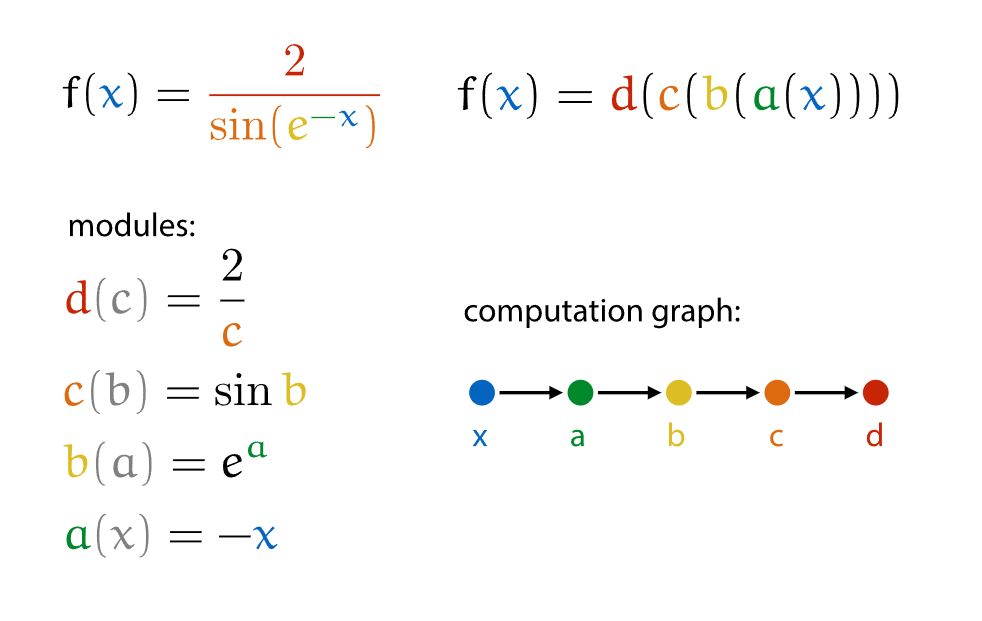
\includegraphics[width=0.5\textwidth]{assets/backpropbasic.png}
\end{figure}

Since we expressed $f(x)$ as a composition we can apply the chain rule, fully written out we get:
\[
    \underbrace{\frac{\partial f}{\partial x}}_{\text{global derivative}} = \underbrace{\frac{\partial d}{\partial c}\frac{\partial c}{\partial b}\frac{\partial b}{\partial a}\frac{\partial a}{\partial x}}_\text{local derivatives}
\]

\subsubsection*{Symbolic computation}

Now all we have to do is work out the derivatives of each module with respect to its inputs. That is, we just calculate the local derivatives of all the module functions.
\[
    \frac{\partial f}{\partial x} = -\frac{2}{c^2}\cdot \cos b \cdot e^a \cdot -1  
\]

\subsubsection*{Numeric computation}

To compute the \textbf{forward pass} we assume some input for $x$ and compute the output of the function $f(x)$ (not the derivative).

\begin{figure}[!h]
    \centering
    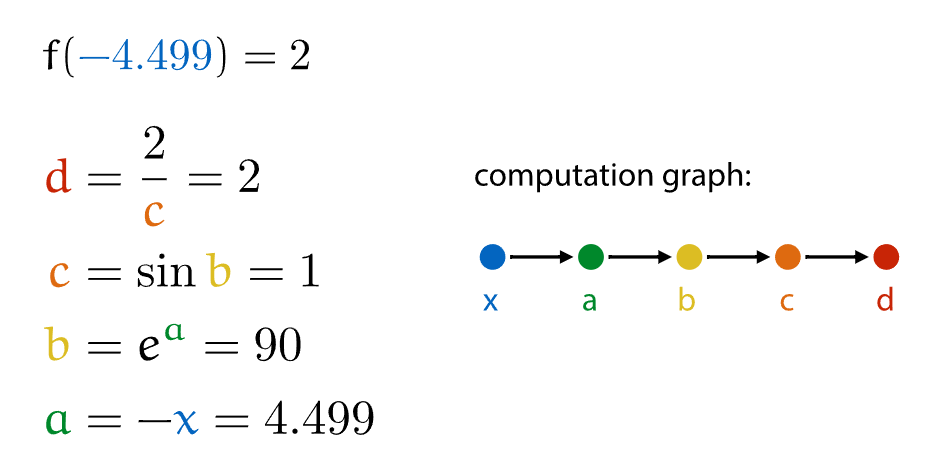
\includegraphics[width=0.5\textwidth]{assets/forwardpass.png}
\end{figure}

To compute the \textbf{backward pass} we take the derivative and populate it with the intermediate values of the module functions from the forward pass. 

\begin{align*}
    \frac{\partial f}{\partial x} & = -\frac{2}{c^2}\cdot \cos b \cdot e^a \cdot -1 \\
    & = -\frac{2}{1^2}\cdot \cos 90 \cdot e^{4.499} \cdot -1 \\
    & = -\frac{1}{2}\cdot 0 \cdot 90 \cdot -1 = 0
\end{align*}

\subsection{Backpropagation in FNN's}

We start off with a FNN with a loss function $l$ and an output node $y$. We describe these two properties as follows (the same FNN as in the pseudocode example):
\begin{align*}
    l & = (y - \text{target})^2 \\
    y & = v_1h_1 + v_2h_2 + v_3h_3 + b_h
\end{align*}

\subsubsection*{Weight update rule for output layer}

If we want to compute the expression to update the weights $v_1, v_2, v_3$ we can use the chain rule to express a change in the loss function with respect to a change in the weights.
\begin{align*}
    \frac{\partial l}{\partial v_i} & = \frac{\partial l}{\partial y}\frac{\partial y}{\partial v_i} \\
    & = 2(y - \text{target})\cdot h_i 
\end{align*}
Using this a single step of stochastic gradient descent for the weight $v_i$ would be:
\[
    v_i \leftarrow v_i - \eta\cdot 2(y - \text{target})\cdot h_i  
\]

\subsubsection*{Weight update rule for hidden layer}
We can apply this idea further by deriving the update rule for the weights from the input to the hidden layer. The hidden layer nodes $h_i$ have outputs that can be expressed as follows: 
\begin{align*}
    h_i & = \sigma(k_i) \\
    k_i & = w_{i1}x_1 + w_{i2}x_2 + b_2
\end{align*}

Once again for the update rule we take the partial derivative of the loss function with respect to the weight we want to update. 
\begin{align*}
    w_{ij} & \leftarrow w_{ij} - \eta\cdot \frac{\partial l}{\partial w_{ij}} \\
    w_{ij} & \leftarrow w_{ij} - \eta\cdot \frac{\partial l}{\partial y}\frac{\partial y}{\partial h_j}\frac{\partial h_j}{\partial k_j}\frac{\partial k_j}{\partial w_{ij}} \quad \text{(chain rule)}\\
    w_{ij} & \leftarrow w_{ij} - \eta\cdot 2(y - \text{target})\cdot v_j\cdot h_j(1-h_j)x_j
\end{align*}

One thing of note is that the term $2(y - \text{target})$ appears in both update rules. This is a common case and this fact can be used to efficiently compute the gradients.

\newpage

\section{Backpropagation and Computation graphs}

\subsection{Computation graphs}

Just as we did in the abstract example we can apply computation graphs to calculating the update rules for FNN's due to their modular structure. An example of a part of a computation graph for a FNN is shown below.

\begin{figure}[!h]
    \centering
    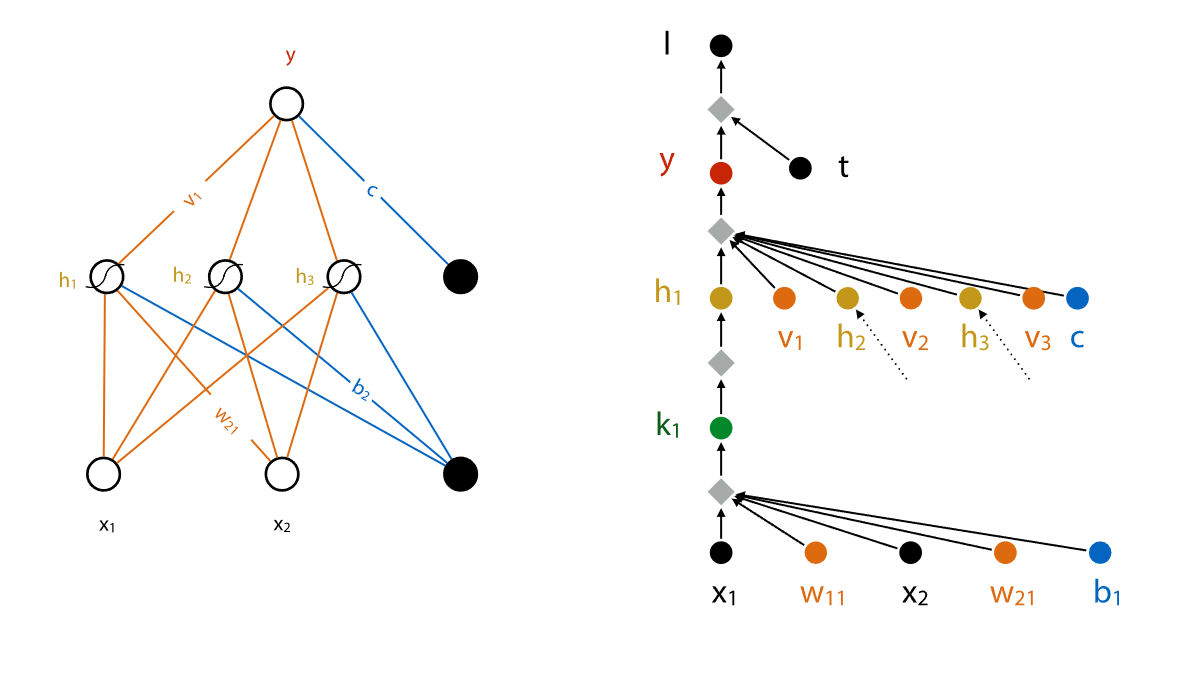
\includegraphics[width=0.6\textwidth]{assets/FNNcompgraph.png}
\end{figure}

Where the nodes can be broken down into two types 
\begin{itemize}[leftmargin=*, noitemsep]
    \item $\diamond$ computation nodes - These nodes represent points where we do computations
    \item $\circ$ variable nodes - These nodes represent the parameters of the model or the model inputs
\end{itemize}

The computations for the diamond nodes are as follows: 
\begin{align*}
    l & = (y - \text{target})^2 \\
    y & = v_1h_1 + v_2h_2 + v_3h_3 + c \\
    h_1 & = \sigma(k_1) \\
    k_1 & = w_{11}x_1 + w_{12}x_2 + b_1
\end{align*}

\subsection{Backpropagation algorithm again}
We can rephrase the abstract backpropagation process now in terms of FNN's and their computation graphs.
\begin{enumerate}[leftmargin=*, noitemsep]
    \item \textbf{forward pass} - We start by doing the forward pass, which means we compute the output of the loss given the inputs to the FNN's. 
    \item \textbf{backward pass} - We start at the top of our computation graphs; compute the derivative for \textit{every} node, that is, the derivative of the output with respect to the node. We then work our way down the graph. 
\end{enumerate}
\newpage
\subsection{Backpropagation on the computation graph}

\begin{multicols}{2}
    \begin{Figure}
        \centering
        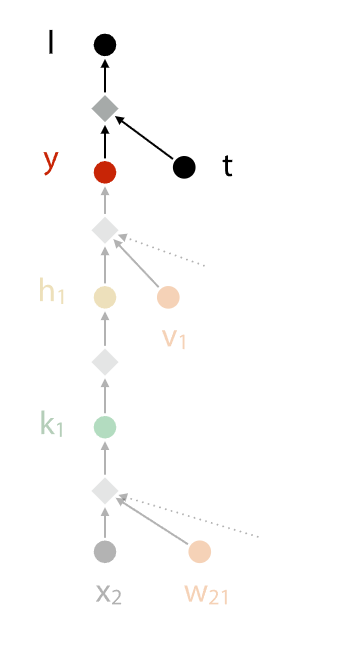
\includegraphics[width=0.4\textwidth]{assets/compgraphtopdown.png}
    \end{Figure}
    \columnbreak 
    We are working top down with the derivatives, so we start off with 
    \[
        \frac{\partial l}{\partial y}=2(y - \text{target})\quad \frac{\partial l}{\partial t}=-2(y - \text{target})
    \]
    The next node is $h_1$ for which the derivative is 
    \[
        \frac{\partial l}{\partial h_1} = \frac{\partial l}{\partial y}\frac{\partial y}{\partial h_1} = 2(y - \text{target})\cdot v_1  
    \]
    An observation to make here is that we already computed $\frac{\partial l}{\partial y}$ so we can use this to compute the derivative of $l$ with respect to $h_1$.
\end{multicols}

\subsubsection*{Precomputed derivatives}

We can express a general rule for the top-down computation of the derivatives, which is that the derivative of the loss with respect to the input generally consists of an already computed derivative times the derivative of the output with respect to the input.
\begin{figure}[!h]
    \centering
    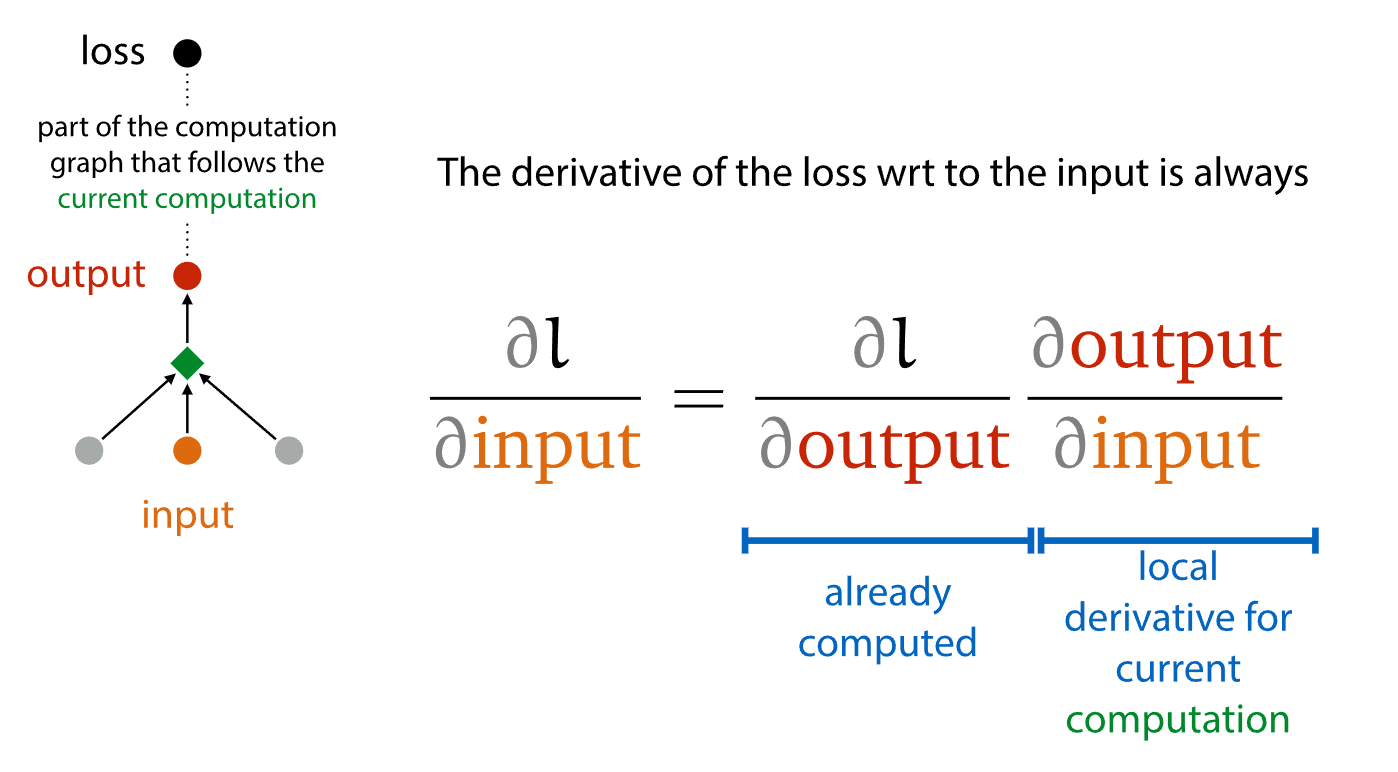
\includegraphics[width=0.4\textwidth]{assets/generalrule.png}
\end{figure}

We can see this property appear again if we want an update rule for $v_1$:
\begin{align*}
    \frac{\partial l}{\partial v_1} & = \frac{\partial l}{\partial y}\frac{\partial y}{\partial v_1} \\
    & = \underbrace{2(y - \text{target})}_\text{already computed}\cdot h_1
\end{align*}
And again if we want the gradient for the weighted sum $k_1$:
\begin{align*}
    \frac{\partial l}{\partial k_1} & = \frac{\partial l}{\partial h_1}\frac{\partial h_1}{\partial k_1} \\
    & = 2(y - \text{target})\cdot v_1\cdot \sigma(k_1)(1-\sigma(k_1)) \\ 
    & = \underbrace{2(y - \text{target})\cdot v_1}_\text{already computed}\cdot h_1(1-h_1)
\end{align*}
And finally again if we want the update rule for $w_{21}$: 
\begin{align*}
    \frac{\partial l}{\partial w_{21}} & = \frac{\partial l}{\partial k_1}\frac{\partial k_1}{\partial w_{21}} \\
    & = \frac{\partial l}{\partial k_1}x_2
\end{align*}

\subsection{Backpropagation full algorithm (fr this time)}
\subsubsection*{Algorithm in english}
\begin{enumerate}[leftmargin=*, noitemsep]
    \item Break your function into a computation graph, make sure the last node is the loss function
    \item Do a forward pass through the graph, computing the output of the loss function
    \item At each \textbf{input} to a \textbf{computation}, multiply 
    \begin{itemize}[leftmargin=*, noitemsep]
        \item the derivative of the loss over the output (already computed)
        \item the derivative of the output over the input 
    \end{itemize}
    \item[$\Rightarrow$] This produces the derivative of the loss over the input
\end{enumerate}
\subsubsection*{Algorithm in pseudocode}

\begin{multicols}{2}
    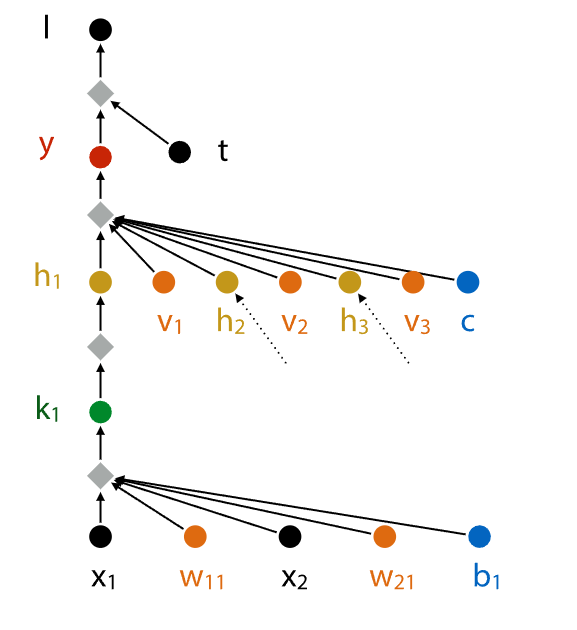
\includegraphics[width=0.35\textwidth]{assets/compgraph2.png}
    \columnbreak
    \begin{lstlisting}
    dy = 2(y - target) # $\partial l / \partial y$
    for i in 1 ... 3: 
        d$v_i$ = dy * $h_i$ 
        d$h_i$ = dy * $v_i$ 
    dc = dy

    for i in 1 ... 3: 
        d$k_i$ = d$h_i$ * $h_i$ * (1 - $h_i$)

    for j in 1 ... 3: 
        for i in 1 ... 2: 
            d$w_{ij}$ = d$k_j$ * $x_i$
        d$b_j$ = d$k_j$
    \end{lstlisting}
\end{multicols}


\end{document}
